\FloatBarrier
\Needspace{12\baselineskip}
\section{评估与结果}
\label{sec:evaluation}
评估检查两种改进：稿件在持续修订中如何变化，研究策略在演化后取得怎样的结果。回应评分预测另行测试，用于判断反馈组件是否能识别已有回应之后的评分变化。

\FloatBarrier
\subsection{评估协议：尝试、稿件与通过分别计数}
\label{sec:protocol}
本次统计在查看档案后选取 G0 初始化及 G1--G3 三代演化作为展示窗口，档案还包含后续代。该阶段共记录 64 次研究尝试、630 次研究调用、28 个完成稿件和 15 个最佳保留版本的模型评阅通过结果。失败与未完成稿件的尝试全部计入总数。\src{10}

\begin{table}[H]
\centering\small
\begin{tabularx}{\textwidth}{P{35mm}Y}
\toprule
\rowcolor{warm}
\textbf{单位或定义} & \textbf{在本报告中的含义}\\
\midrule
研究尝试（episode） & 一次完整研究执行，失败也进入总数和调用统计\\
研究调用 & 历史驱动器记录的研究阶段执行器启动次数\\
完成稿件 & 产生所要求的稿件产物；与评阅通过分开记录\\
当前轮通过 & 该评分轮正在评阅的版本满足历史 Accept 规则\\
最佳保留版本通过 & 最高均分版本恢复后，采用该版本的评价标签\\
固定内循环子集 & 同一组 28 个完成稿件，跟踪初评与三轮修订\\
策略比较批次 & 每代初始策略与所选策略各对应四次研究尝试\\
\bottomrule
\end{tabularx}
\caption{数学评估的单位与版本口径。完成、当前轮通过和最佳版本通过分别回答不同问题。}
\label{tab:protocol}
\end{table}

\Sub{历史评阅与版本恢复}
历史评阅每轮启动三个新 Codex 会话，按 SAC 模拟量表评价稿件，至少一票 Accept 即记为通过。初评之后进行三轮修订与再评阅，最终恢复平均评分最高的版本，并采用它的评价标签。这里的通过指历史模型评阅通过，与真实会议录用及当前可移植版本的固定终审分别处理。

稿件修订只跟踪已经完成的 28 个稿件；失败和未完成尝试保留在外循环统计中。每代初始策略与所选策略的批次各含四次尝试，其中 G0、G1 的两个角色指向同一批次，总账中只计一次。

\Sub{策略比较与调用覆盖}
历史策略会从给定方向中自主选择具体目标，比较结果因此包含选题与执行做法的共同影响。各批次为自适应、非配对的历史运行，未预选同一命题，也未设置等 token、美元或人时预算及演化算子消融。我们分别列出所选策略、整代种群与整个窗口的计数，使采用一个策略和搜索策略的投入都能被看到。

调用账本包括研究阶段启动、独立评阅会话，以及根据非初轮评分推算的修订尝试。每组评阅包含三个独立会话，合计时按会话计数，组数不重复相加。合计调用数是成本代理，尚未覆盖策略教练与育种、内部模型及工具调用、未记录重试、完整计费 token、美元和主动人时。

\Sub{过程证据与预测指标}
问题筛选案例 E1 来自早期分阶段复判，回应两轮记录采用历史内部代理停止规则。它们展示执行过程中的判断变化。回应预测则使用既有论文、评审与回应，以最终评分减初始评分的符号为标签。数学统计可由公开聚合数据核对；回应预测保留来源报告的指标值。评价协议随报告公开。

\FloatBarrier
\subsection{稿件修订：当前通过数从 3 增至 12}
\label{sec:inner-results}
同一组 28 个完成稿件经历初评与三轮修订，当前通过数依次为 3、10、10、12，均分由约 4.65 升至 5.67。图\ref{fig:inner} 展示当前版本轨迹，表\ref{tab:rounds} 同时列出截至各轮的最佳保留版本。

\Fig{\earfigure{inner_progress}}{G0--G3 的固定 28 稿件子集。图展示初评及三轮修订中当前版本的通过数与平均评分；各轮最佳保留版本结果见表\ref{tab:rounds}。}{fig:inner}

\begin{table}[H]
\centering\small
\begin{tabularx}{\textwidth}{P{22mm}YYYY}
\toprule
\rowcolor{warm}
\textbf{评分轮} & \textbf{当前通过数} & \textbf{当前均分} & \textbf{最佳保留通过数} & \textbf{最佳保留均分}\\
\midrule
初评 & 3 & 4.648 & 3 & 4.648\\
修订 1 & 10 & 5.247 & 10 & 5.270\\
修订 2 & 10 & 5.498 & 12 & 5.568\\
修订 3 & 12 & 5.675 & 15 & 5.790\\
\bottomrule
\end{tabularx}
\caption{固定稿件子集的逐轮结果。每轮均为 28 个稿件；均分展示到三位小数，完整聚合值保存在发布数据中。均分由来源记录的分数和复算。}
\label{tab:rounds}
\end{table}

当前通过比例由 $3/28=10.7\%$ 增至 $12/28=42.9\%$，初末均分差约 1.03。最后轮与初轮相比，27 个稿件均分提高、1 个下降。修订后，这组稿件的模型评阅结果整体改善；记录尚未设置仅重新评分的对照，因而不能单独估计依据反馈修订的因果收益。\src{10}

\Sub{保留最高均分版本，处理修订中的回落}
版本轨迹中也有回落。13 个稿件的最后轮均分低于各自历史最佳均分，3 个稿件的最佳版本通过、最后轮未通过。恢复最高均分版本后，最终保留稿件的通过数为 15；最后轮当前通过数为 12。这些回落说明了保留版本历史的实际作用：修订继续进行，已有的较好稿件仍能交付。

\FloatBarrier
\subsection{G3 所选策略：更多通过，更少研究调用}
\label{sec:strategy-results}
各代所选策略的历史通过率见图\ref{fig:evolution}。每个点对应四次完整研究尝试，失败和未完成尝试也在分母中。G0、G1 的所选批次均无通过结果，G2 为 $2/4$，G3 为 $3/4$；各代使用分别选出的策略及研究目标。

\Fig{\earfigure{evolution_progress}}{G0 初始化及 G1--G3 三代演化中，所选策略通过率依次为 0\%、0\%、50\%、75\%。各点为四次历史研究尝试；不是同一策略在固定任务上的连续测量。}{fig:evolution}

\Sub{把上一轮遇到的问题，变成下一轮的改法}
外循环把退出原因与评阅意见带回策略修改。历史记录中的改动包括缩短候选清单、提前要求核心引理与证明路线，以及提高贡献要求。后续批次再用研究结果检验这些做法。表\ref{tab:strategy-batches} 列出初始与所选策略的批次计数，表\ref{tab:population} 列出全部候选的种群总账。

\begin{table}[H]
\centering\small
\begin{tabularx}{\textwidth}{P{13mm}YYYY}
\toprule
\rowcolor{warm}
\textbf{代} & \textbf{初始通过／尝试} & \textbf{所选通过／尝试} & \textbf{初始研究调用} & \textbf{所选研究调用}\\
\midrule
G0 & 0/4 & 0/4 & 53 & 53\\
G1 & 0/4 & 0/4 & 40 & 40\\
G2 & 0/4 & 2/4 & 24 & 45\\
G3 & 2/4 & 3/4 & 41 & 29\\
\bottomrule
\end{tabularx}
\caption{初始策略与每代所选策略的历史批次比较。G0、G1 的两个角色指向同一批次，不能重复计入完整种群。}
\label{tab:strategy-batches}
\end{table}

\begin{table}[H]
\centering\small
\begin{tabularx}{\textwidth}{P{15mm}YYYYY}
\toprule
\rowcolor{warm}
\textbf{代} & \textbf{尝试} & \textbf{研究调用} & \textbf{完成稿件} & \textbf{最佳版本通过} & \textbf{通过率}\\
\midrule
G0 & 12 & 169 & 1 & 0 & 0.0\%\\
G1 & 16 & 155 & 5 & 1 & 6.25\%\\
G2 & 16 & 148 & 8 & 5 & 31.25\%\\
G3 & 20 & 158 & 14 & 9 & 45.0\%\\
\midrule
合计 & 64 & 630 & 28 & 15 & 23.4\%\\
\bottomrule
\end{tabularx}
\caption{G0--G3 完整种群计数。失败和未完成尝试保留在分母中，所选批次与整体表现分别报告。}
\label{tab:population}
\end{table}

G3 所选策略通过率为 75\%（$3/4$），初始策略为 50\%（$2/4$）。计入当代全部候选与初始策略后，G3 整代为 45\%（$9/20$）；整个窗口为 $15/64=23.4\%$。只统计完成稿件，则为 $15/28=53.6\%$。采用所选策略、开展策略搜索与完成稿件后的评价，对应这三种不同的统计范围。

\Sub{每个通过结果，研究调用减少 52.8\%}
G3 的两个策略批次各执行四次研究尝试。初始策略使用 41 次研究调用，得到 2 个通过结果；所选策略使用 29 次，得到 3 个通过结果。图\ref{fig:cost} 与表\ref{tab:cost} 将研究、评阅和推算修订放在同一账本中。

\begin{figure}[H]
\centering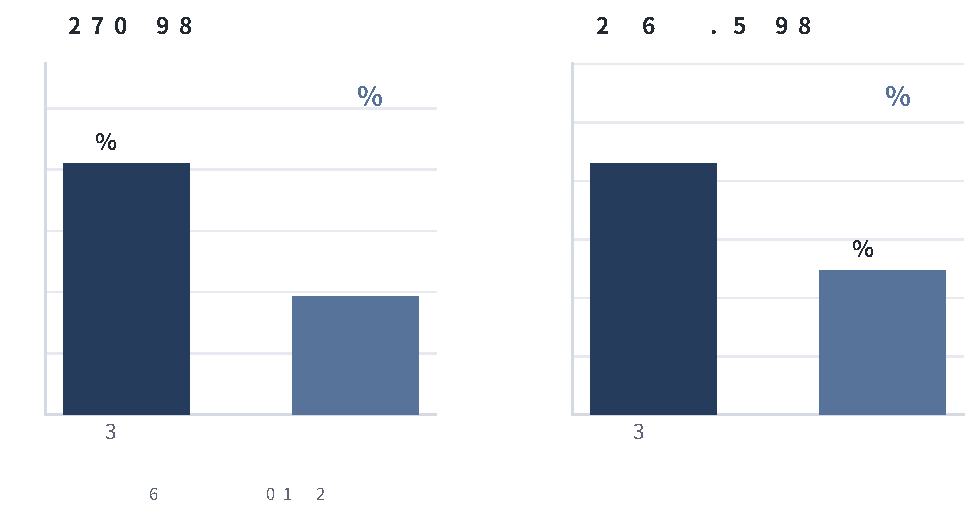
\includegraphics[width=.88\textwidth]{../../figures/cn/cost_comparison.pdf}
\caption{G3 每通过结果的研究调用由 $41/2=20.50$ 降至 $29/3=9.67$，减少 52.8\%；研究、评阅和推算修订的合计代理由 $86/2=43.00$ 降至 $74/3=24.67$，减少 42.6\%。}
\label{fig:cost}
\end{figure}

\begin{table}[H]
\centering\small\setlength{\tabcolsep}{3pt}
\begin{tabularx}{\textwidth}{P{21mm}rrrrrY}
\toprule
\rowcolor{warm}
\textbf{G3 策略} & \textbf{研究} & \textbf{评阅} & \textbf{修订$^*$} & \textbf{合计} & \textbf{通过} & \textbf{合计／通过}\\
\midrule
初始策略 & 41 & 36 & 9 & 86 & 2 & 43.00\\
所选策略 & 29 & 36 & 9 & 74 & 3 & 24.67\\
\bottomrule
\end{tabularx}
\caption{G3 调用账本，每组四次研究。两个策略批次各有 12 组评阅、36 个独立会话；修订$^*$由非初轮评分推算，评阅组数不重复加入合计。}
\label{tab:cost}
\end{table}

每次研究尝试的研究调用由 $41/4=10.25$ 降至 $29/4=7.25$，通过数同时由 2 增至 3，共同带来每通过研究调用下降 52.8\%。计入评阅与推算修订后，合计代理每通过下降 42.6\%。两项比值的统计范围见第\ref{sec:protocol} 节，完整机器费用与人时尚未计入。

把整个搜索过程计入，G0--G3 累计 630 次研究调用和 15 个通过结果，研究调用每通过为 42。这个总账包含寻找策略的投入，与采用 G3 所选策略批次的成本分别报告。零通过批次的每通过调用无定义。

\Sub{通过定义影响策略比较的解读}
我们还用保留的评阅票做了一项更严格的诊断：要求三票均 Accept，且每票评分至少 7。G3 初始与所选策略都只有 $1/4$ 次尝试满足要求。该诊断未重新评阅，说明历史通过规则会影响优势的解读。小批次、自选目标与事后选定的展示窗口，也限制了结果的推广范围；稳定收益仍需匹配任务、统一质量检查和完整资源核算来验证。\src{10}

\FloatBarrier
\Needspace{185mm}
\subsection{评分预测：提分与不变可辨，降分仍难判}
\label{sec:rebuttal-results}
回应反馈评价器读取论文、初始评阅与作者当时的回应，预测评分上涨、不变或下降。每个案例单独输入模型，最终评分仅用于核对标签，实际变化写为 $\operatorname{sign}(R_{\mathrm{final}}-R_{\mathrm{initial}})$。

测试连接公开 OpenReview 历史记录与 ProReviewer 初始评分，采用 DeepSeek V4 Pro、案例隔离、零样本提示和 temperature 0。表\ref{tab:rebuttal-eval} 列出来源报告的聚合结果。Macro-F1 为各类别 F1 的平均，越接近 1 越好。\src{1,8,10}

\begin{table}[H]
\centering\small
\begin{tabularx}{\textwidth}{P{31mm}Y P{19mm}}
\toprule
\rowcolor{warm}
\textbf{来源与样本} & \textbf{预测设置} & \textbf{Macro-F1}\\
\midrule
36 例均衡子集 & 上涨与不变各 18 例，不含下降类 & 0.805\\
57 例完整测试 & 上涨、不变和下降三类，含 6 例下降 & 0.503\\
同一 57 例来源集 & 来源报告的上涨／不变二类指标$^*$ & 0.755\\
\bottomrule
\end{tabularx}
\caption{回应评分变化预测。$^*$第三行来自同一 57 例来源集，有效二类样本分母未单列；三行分别对应不同评价设置。F1 保留来源报告值，公开材料尚不含可重新估计的逐例预测。}
\label{tab:rebuttal-eval}
\end{table}

36 例均衡二类测试的 Macro-F1 为 0.805；57 例完整三类测试为 0.503，其中下降类 F1 为 0。下降类识别是这一评价器的明显弱点，二类测试中的区分能力无法覆盖它。进一步修改提示未改善留出集表现，因此保留原始零样本提示，未修改模型权重。

EAR 用评分变化预测与证据检查比较草稿。当前测试回答的是能否预测既有回应之后的评分变化；生成的新回应是否提高真实审稿人的评分，还需要单独实验。实际回应决策仍须结合内容、证据和作者判断，尤其要注意评价器对下降类的识别不足。

\Sub{公开材料与结果核对}
公开的计数、分数和及评价协议，可以核对均值、比例、调用总数与每通过成本。匿名过程记录保留了证据改变决策、反馈改变策略的具体转折。公开聚合材料尚不包含个别研究目标、完整稿件、逐票文本、逐例回应预测与完整执行日志；它支持统计核对，完整研究过程的复现还需要这些材料。
